\section{Auswertung}
\label{sec:Auswertung}
%Hier kannst du ja noch einen Satz schreiben, wenn du möchtest xD
Für den Fehler $\Delta N$ der gemessenen Teilchen $N$ gilt
\begin{equation*}
    \Delta N = \sqrt{N} \,,
\end{equation*}
da radioaktive Zerfälle poissonverteilt sind.

%\subsection{$\gamma$-Strahler}
\subsection{Gamma-Strahler}
\label{sec:Gamma-Strahler}



Bei der zu Beginn über einen Zeitraum von $t = 900 \,\unit{\second}$ durchgeführten Nullmessung wurden
\begin{equation*}
    N_0  = 845 \pm 29
\end{equation*}
Ereignisse gemessen.
Das entspricht einer Ruheaktivität von
\begin{equation*}
    A_0 = (0.94 \pm 0.032) \,\dfrac{1}{\unit{\second}} \, .
\end{equation*}

In der \autoref{tab:gammablei} sind die Messdaten der ersten Messreihe, also mit Bleiplatten als Absorbermaterial, angegeben.
\begin{table}[H]
    \centering
    \caption{Messwerte zum $\gamma$-Strahler mit Bleiabschirmung.}
    \label{tab:gammablei}
    \begin{tabular}{S[table-format=2.2] S[table-format=5.0] S[table-format=3.0] S}
      \toprule
      {$D \mathbin{/} \unit{\milli\meter} $} & {$\text{Teilchenzahl}$} & {$\text{Zeit} \,t \mathbin{/} \unit{\second}$} &{$ \left(\text{A}- \text{A}_0 \right) \mathbin{/} \unit{\frac{1}{\second}}$} \\
      \midrule
       1.40   &{$ 10708 \pm  103,47  $}& 100 & {$106,14   \pm 1,03$}  \\
       1.24  & {$10348  \pm  101,72  $}& 100 & {$102,54   \pm 1,03$}  \\
       1.18  & {$ 9906  \pm  99,52  $}& 100 & {$ 98,12   \pm 0,10$}  \\
       1.34  & {$10048  \pm  100,23  $}& 100 & {$ 99,54   \pm 1,00$}  \\
       1.16  & {$10071  \pm  100,35  $}& 100 & {$ 99,77   \pm 1,00$}  \\
       1.26  & {$10430  \pm  102,12  $}& 100 & {$103,36   \pm 1,02$}  \\
       1.14  & {$10182  \pm  100,90  $}& 100 & {$100,88   \pm 1,01$}  \\
      10.18  & {$ 8357  \pm  91,41   $}& 200 & {$ 40,85   \pm 0,46$}  \\
      10.20  & {$ 9043  \pm  95,09   $}& 200 & {$ 44,28   \pm 0,48$}  \\
      20.10  & {$ 3375  \pm  58,09  $}& 200 & {$ 15,94   \pm 0,29$}  \\
      \bottomrule
    \end{tabular}
  \end{table}

Zunächst wird die Hintergrundaktivität von der gemessen Aktivität abgezogen.
Die so bereinigten Messdaten aus \autoref{tab:gammablei} werden in einem halblogarithmischem Diagramm aufgetragen und es wird, wie in \autoref{fig:plot1} zu erkennen, eine Ausgeleichsfunktion berechnet.

\begin{figure}[H]
    \centering
    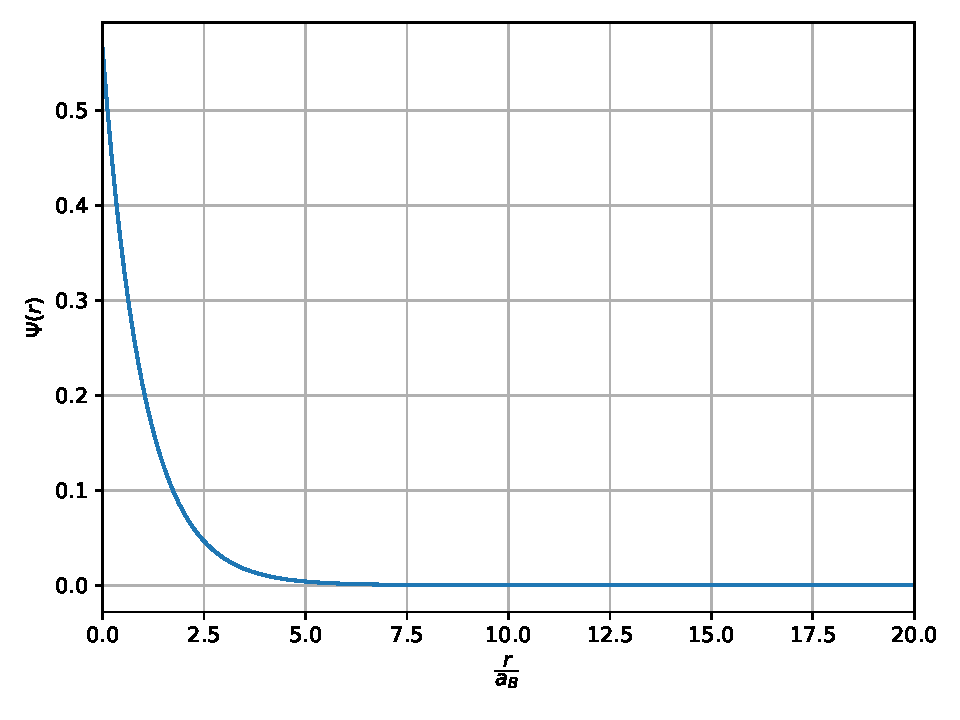
\includegraphics{Graph_a.pdf}
    \caption{Ausgeleichsfunktion zur Bestimmung des Absorptionskoeffizienten mit Bleiabsorber.}
    \label{fig:plot1}
  \end{figure}

Aus der Ausgleichsrechung wird der Absorptionskoeffizienten 
\begin{equation*}
    \mu =  \left( 96,958 \pm 5,079 \right) \unit{\dfrac{1}{\meter}}
\end{equation*}
abgelesen. 
Die Anfangsaktvität bzw. der y-Achsenabschnitt, ist mit 
\begin{equation*}
    A =  \left( 111,434 \pm 1,024 \right)  \dfrac{1}{\unit{\second}}
\end{equation*}
gegeben. \\

Analog wird für die zweite Messreihe verfahren.
Dabei sind in \autoref{tab:gammakupfer} die Messdaten für die unterschiedlichen Dicken der Kupferabsorber dargestellt.

\begin{table}[H]
    \centering
    \caption{Messwerte zum $\gamma$-Strahler mit Kupferabsorber.}
    \label{tab:gammakupfer}
    \begin{tabular}{S[table-format=2.2] S[table-format=5.0] S[table-format=3.0] S}
      \toprule
      {$D \mathbin{/} \unit{\milli\meter} $} & {$\text{Teilchenzahl}$} & {$\text{Zeit} \,t \mathbin{/} \unit{\second}$} &{$ \left(\text{A}- \text{A}_0 \right) \mathbin{/} \unit{\frac{1}{\second}}$} \\
      \midrule
      {$ 0,70 \pm 0,02$}          &    {$  10948 \pm 104,63    $} &      100  	& {$108,54  \pm 1,05$} \\
      {$ 0,62 \pm 0,02$}          &    {$  11137 \pm 105,53    $} &      100  	& {$110,43  \pm 1,06$} \\
      {$ 0,51 \pm 0,02$}          &    {$  11065 \pm 105,19    $} &      100  	& {$109,71  \pm 1,05$} \\
      {$ 0,54 \pm 0,02$}          &    {$  10953 \pm 104,66    $} &      100  	& {$108,59  \pm 1,05$} \\
      {$ 4,94 \pm 0,02$}          &    {$  18462 \pm 135,87    $} &      100  	& {$183,68  \pm 1,36$} \\
      {$ 9,94 \pm 0,02$}          &    {$  15284 \pm 123,63    $} &      100  	& {$75,856  \pm 0,62$} \\
      {$20,00 \pm 0,02$}          &    {$   9863 \pm 99,31     $} &      200  	& {$ 48,38  \pm 0,50$} \\
      {$20,10 \pm 0,02$}          &    {$  10257 \pm 101,28    $} &      200  	& {$ 50,35  \pm 0,51$} \\
      \bottomrule
    \end{tabular}
  \end{table}

  Erneut werden die aufgenommenen Ereignisse grafisch aufgetragen und es wird eine Ausgleichsrechung durchgeführt, sodass der in \autoref{fig:plot2} zu erkennende Plot entsteht.

  \begin{figure}[H]
      \centering
      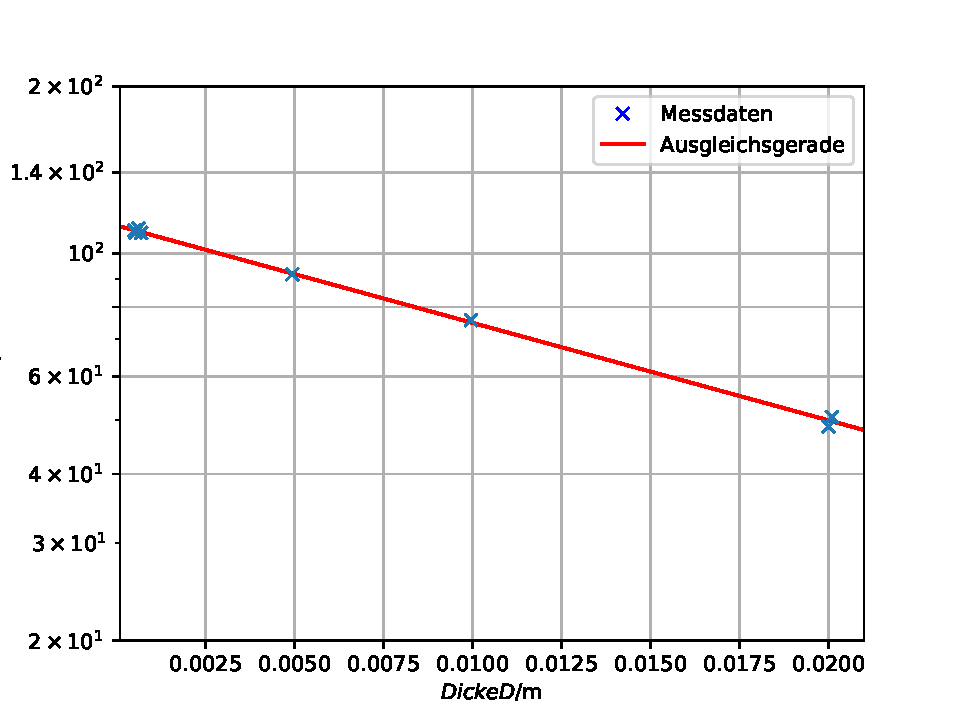
\includegraphics{figures/GammaKupfer2.pdf}
      \caption{Ausgeleichsfunktion zur Bestimmung des Absorptionskoeffizienten mit Kupferabsorber.}
      \label{fig:plot2}
  \end{figure}

Hier ergibt sich der Absorptionskoeffizient zu
\begin{equation*}
    \mu =  \left(40,481 \pm 0,681\right) \unit{\frac{1}{\meter}}
\end{equation*}
und die Anfangsaktivität zu
\begin{equation*}
    A = (112,295 \pm 1.00) \, \unit{\frac{1}{\second}} \,.
\end{equation*}

Verglichen mit einem Theoriewert von % Hast du den Theoriewert irgendwo?

\begin{equation*}
    \mu_{\text{theo}} = 63,2  \dfrac{1}{\unit{\meter}} \,.%sorry, aber ich habe echt keine Ahnung wie man den berechnen soll
\end{equation*}

%\subsection*{$\beta$-Strahler}
\subsection{Beta-Strahler}
\label{sec:Beta-Strahler}

Mithilfe der in \autoref{tab:beta} dargestellten Werte Wird erneut eine Regressionsrechnung durchgeführt. 

Bei der zu Beginn über einen Zeitraum von $t = 900 \,\unit{\second}$ durchgeführten Nullmessung wurden
\begin{equation*}
    N_0  = 579 \pm 24
\end{equation*}
und die Nullaktivät

\begin{equation*}
    A_0  = 0,643 \pm 0,027 \dfrac{1}{\unit{\second}} \, .
\end{equation*}

\begin{table}[H]
    \centering
    \caption{Messwerte zum $\beta$-Strahler.}
    \label{tab:beta}
    \begin{tabular}{S[table-format=3.0] S[table-format=5.0] S[table-format=3.0] S}
      \toprule
      {$D \mathbin{/} \unit{\micro\meter} $} & {$\text{Teilchenzahl}$} & {$\text{Zeit} \,t \mathbin{/} \unit{\second}$} &{$ \left(\text{A}- \text{A}_0 \right) \mathbin{/} \unit{\frac{1}{\second}}$} \\
      \midrule
      {$482 \pm 1,0$}      &         {$339 \pm 18,41$ }    &       500  &  0,035 \pm 0,005 \\
      {$444 \pm 2,0$}      &         {$335 \pm 18,30$ }    &       500  &  0,027 \pm 0,004 \\
      {$400 \pm 1,0$}      &         {$338 \pm 18,38$ }    &       500  &  0,033 \pm 0,004 \\
      {$338 \pm 5,0$}      &         {$293 \pm 17,11$ }    &       400  &  0,089 \pm 0,011 \\
      {$302 \pm 1,0$}      &         {$324 \pm 18,00$ }    &       400  &  0,167 \pm 0,013 \\
      {$253 \pm 1,0$}      &         {$228 \pm 15,09$ }    &       300  &  0,117 \pm 0,018 \\
      {$200 \pm 1,0$}      &         {$655 \pm 25,59$ }    &       300  &  1,540 \pm 0,053 \\
      {$160 \pm 1,0$}      &        {$1207 \pm 34,74$}     &       200  &  5,392 \pm 0,141 \\
      {$152 \pm 0,5$}      &        {$1957 \pm 44,23$}     &       200  &  9,142 \pm 0,189 \\
      {$125 \pm 0,0$}      &        {$1906 \pm 43,65$}     &       200  &  8,887 \pm 0,186 \\
      {$100 \pm 0,0$}      &        {$8006 \pm 89,47$}     &       200  & 39,387 \pm 0,415 \\
      \bottomrule
    \end{tabular}
  \end{table}

Wie in \autoref{fig:plot3} zu erkennen, wird dabei die Massenbelegung $R$ halblogarithmisch gegen die Aktivität $A - A_0$ geplottet.
\begin{figure}[H]
    \centering
    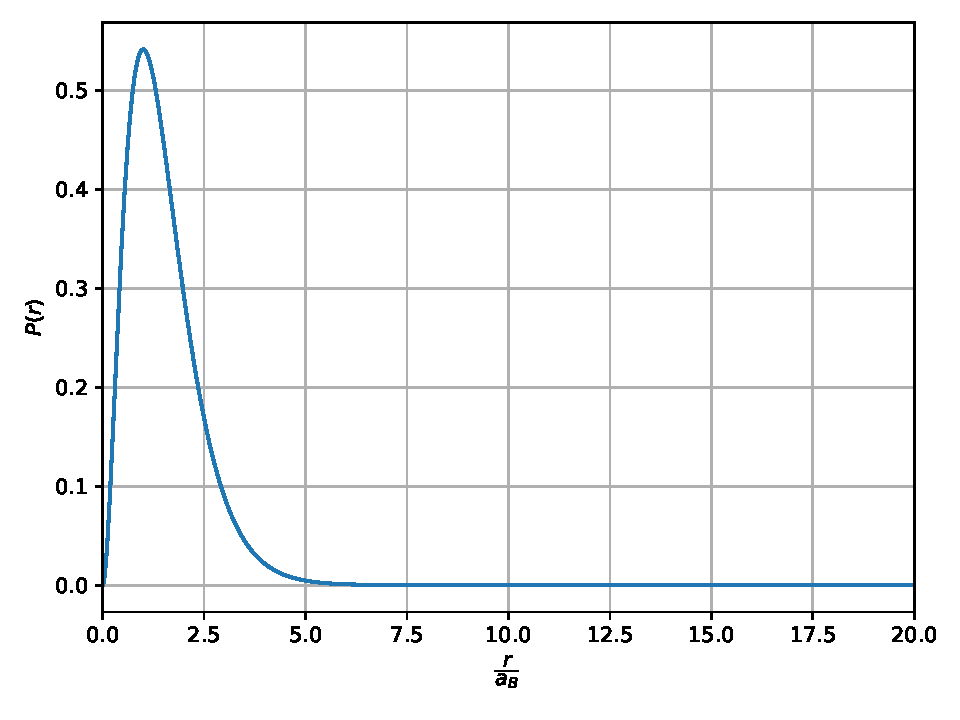
\includegraphics{build/Graph_c.pdf}
    \caption{Durchgehende Strahlungsintensität und Untergrundstrahlung in Abhängigkeit der Massenbelegung $R$.}
    \label{fig:plot3}
\end{figure}
Die beiden eingezeichneten Geraden stellen die durchgehende Strahlungsintensität sowie die Untergrundstrahlung dar. \\
Dabei ist die Gesamtreichweite $R_\text{max}$ der Strahlung durch
\begin{equation*}
    R_\text{max} = \frac{b_2 - b_1}{m_1 - m_2}
\end{equation*}
gegeben, wobei $b_i$ die y-Achsenabschnitte und $m_i$ die Steigungen der beiden Geraden repräsentieren. \\

Mit
%\begin{align*}
%    m_1 &= -14.51 \dfrac{\unit{\kilo\gram}{\unit{\second \meter^2}}}    \\
%    m_2 &= -0.28  \dfrac{\unit{\kilo\gram}{\unit{\second \meter^2}}}    \\
%    b_1 &= 1958.80  \dfrac{1}{\unit{\second}}                           \\
%    b_2 &= 0.95     \dfrac{1}{\unit{\second}}                           \\
%\end{align*} ergibt sich

\begin{align*}
    m_1 &= -14,51  \pm 3,38\,  \dfrac{\unit{\kilo\gram}}{\unit{\second \cdot \meter^2}}\\
    m_2 &= -0,28   \pm 0,09\,  \dfrac{\unit{\kilo\gram}}{\unit{\second \cdot \meter^2}}  \\
    b_1 &= 1958,80 \pm 0,96\,  \dfrac{1}{\unit{\second}}                         \\
    b_2 &= 0,95    \pm 0,09\,  \dfrac{1}{\unit{\second}}                          \\
\end{align*} ergibt sich

\begin{equation*}
    R_\text{max} = \left( 0,54 \pm 0,14 \right)  \unit{\meter} \,.
\end{equation*}

und damit nach \eqref{eq:Emax} eine Maximalenergie von
\begin{equation*}
    E_\text{max} = \left(1,22 \pm 0,28 \right) \, \unit{\mega\eV} \,.
\end{equation*}


